\documentclass[]{article}
\usepackage{lmodern}
\usepackage{amssymb,amsmath}
\usepackage{ifxetex,ifluatex}
\usepackage{fixltx2e} % provides \textsubscript
\ifnum 0\ifxetex 1\fi\ifluatex 1\fi=0 % if pdftex
  \usepackage[T1]{fontenc}
  \usepackage[utf8]{inputenc}
\else % if luatex or xelatex
  \ifxetex
    \usepackage{mathspec}
  \else
    \usepackage{fontspec}
  \fi
  \defaultfontfeatures{Ligatures=TeX,Scale=MatchLowercase}
\fi
% use upquote if available, for straight quotes in verbatim environments
\IfFileExists{upquote.sty}{\usepackage{upquote}}{}
% use microtype if available
\IfFileExists{microtype.sty}{%
\usepackage{microtype}
\UseMicrotypeSet[protrusion]{basicmath} % disable protrusion for tt fonts
}{}
\usepackage[margin=1in]{geometry}
\usepackage{hyperref}
\hypersetup{unicode=true,
            pdftitle={Causal Inference Final Project: Effect of Smoking on 10-year Development of Coronary Heart Disease},
            pdfauthor={Bianca Doone, Michael Attah, Graham Casey Gibson, Daniel Saunders, Nutcha Wattanachit},
            pdfborder={0 0 0},
            breaklinks=true}
\urlstyle{same}  % don't use monospace font for urls
\usepackage{color}
\usepackage{fancyvrb}
\newcommand{\VerbBar}{|}
\newcommand{\VERB}{\Verb[commandchars=\\\{\}]}
\DefineVerbatimEnvironment{Highlighting}{Verbatim}{commandchars=\\\{\}}
% Add ',fontsize=\small' for more characters per line
\usepackage{framed}
\definecolor{shadecolor}{RGB}{248,248,248}
\newenvironment{Shaded}{\begin{snugshade}}{\end{snugshade}}
\newcommand{\KeywordTok}[1]{\textcolor[rgb]{0.13,0.29,0.53}{\textbf{#1}}}
\newcommand{\DataTypeTok}[1]{\textcolor[rgb]{0.13,0.29,0.53}{#1}}
\newcommand{\DecValTok}[1]{\textcolor[rgb]{0.00,0.00,0.81}{#1}}
\newcommand{\BaseNTok}[1]{\textcolor[rgb]{0.00,0.00,0.81}{#1}}
\newcommand{\FloatTok}[1]{\textcolor[rgb]{0.00,0.00,0.81}{#1}}
\newcommand{\ConstantTok}[1]{\textcolor[rgb]{0.00,0.00,0.00}{#1}}
\newcommand{\CharTok}[1]{\textcolor[rgb]{0.31,0.60,0.02}{#1}}
\newcommand{\SpecialCharTok}[1]{\textcolor[rgb]{0.00,0.00,0.00}{#1}}
\newcommand{\StringTok}[1]{\textcolor[rgb]{0.31,0.60,0.02}{#1}}
\newcommand{\VerbatimStringTok}[1]{\textcolor[rgb]{0.31,0.60,0.02}{#1}}
\newcommand{\SpecialStringTok}[1]{\textcolor[rgb]{0.31,0.60,0.02}{#1}}
\newcommand{\ImportTok}[1]{#1}
\newcommand{\CommentTok}[1]{\textcolor[rgb]{0.56,0.35,0.01}{\textit{#1}}}
\newcommand{\DocumentationTok}[1]{\textcolor[rgb]{0.56,0.35,0.01}{\textbf{\textit{#1}}}}
\newcommand{\AnnotationTok}[1]{\textcolor[rgb]{0.56,0.35,0.01}{\textbf{\textit{#1}}}}
\newcommand{\CommentVarTok}[1]{\textcolor[rgb]{0.56,0.35,0.01}{\textbf{\textit{#1}}}}
\newcommand{\OtherTok}[1]{\textcolor[rgb]{0.56,0.35,0.01}{#1}}
\newcommand{\FunctionTok}[1]{\textcolor[rgb]{0.00,0.00,0.00}{#1}}
\newcommand{\VariableTok}[1]{\textcolor[rgb]{0.00,0.00,0.00}{#1}}
\newcommand{\ControlFlowTok}[1]{\textcolor[rgb]{0.13,0.29,0.53}{\textbf{#1}}}
\newcommand{\OperatorTok}[1]{\textcolor[rgb]{0.81,0.36,0.00}{\textbf{#1}}}
\newcommand{\BuiltInTok}[1]{#1}
\newcommand{\ExtensionTok}[1]{#1}
\newcommand{\PreprocessorTok}[1]{\textcolor[rgb]{0.56,0.35,0.01}{\textit{#1}}}
\newcommand{\AttributeTok}[1]{\textcolor[rgb]{0.77,0.63,0.00}{#1}}
\newcommand{\RegionMarkerTok}[1]{#1}
\newcommand{\InformationTok}[1]{\textcolor[rgb]{0.56,0.35,0.01}{\textbf{\textit{#1}}}}
\newcommand{\WarningTok}[1]{\textcolor[rgb]{0.56,0.35,0.01}{\textbf{\textit{#1}}}}
\newcommand{\AlertTok}[1]{\textcolor[rgb]{0.94,0.16,0.16}{#1}}
\newcommand{\ErrorTok}[1]{\textcolor[rgb]{0.64,0.00,0.00}{\textbf{#1}}}
\newcommand{\NormalTok}[1]{#1}
\usepackage{longtable,booktabs}
\usepackage{graphicx,grffile}
\makeatletter
\def\maxwidth{\ifdim\Gin@nat@width>\linewidth\linewidth\else\Gin@nat@width\fi}
\def\maxheight{\ifdim\Gin@nat@height>\textheight\textheight\else\Gin@nat@height\fi}
\makeatother
% Scale images if necessary, so that they will not overflow the page
% margins by default, and it is still possible to overwrite the defaults
% using explicit options in \includegraphics[width, height, ...]{}
\setkeys{Gin}{width=\maxwidth,height=\maxheight,keepaspectratio}
\IfFileExists{parskip.sty}{%
\usepackage{parskip}
}{% else
\setlength{\parindent}{0pt}
\setlength{\parskip}{6pt plus 2pt minus 1pt}
}
\setlength{\emergencystretch}{3em}  % prevent overfull lines
\providecommand{\tightlist}{%
  \setlength{\itemsep}{0pt}\setlength{\parskip}{0pt}}
\setcounter{secnumdepth}{0}
% Redefines (sub)paragraphs to behave more like sections
\ifx\paragraph\undefined\else
\let\oldparagraph\paragraph
\renewcommand{\paragraph}[1]{\oldparagraph{#1}\mbox{}}
\fi
\ifx\subparagraph\undefined\else
\let\oldsubparagraph\subparagraph
\renewcommand{\subparagraph}[1]{\oldsubparagraph{#1}\mbox{}}
\fi

%%% Use protect on footnotes to avoid problems with footnotes in titles
\let\rmarkdownfootnote\footnote%
\def\footnote{\protect\rmarkdownfootnote}

%%% Change title format to be more compact
\usepackage{titling}

% Create subtitle command for use in maketitle
\newcommand{\subtitle}[1]{
  \posttitle{
    \begin{center}\large#1\end{center}
    }
}

\setlength{\droptitle}{-2em}
  \title{Causal Inference Final Project: Effect of Smoking on 10-year Development
of Coronary Heart Disease}
  \pretitle{\vspace{\droptitle}\centering\huge}
  \posttitle{\par}
  \author{Bianca Doone, Michael Attah, Graham Casey Gibson, Daniel Saunders,
Nutcha Wattanachit}
  \preauthor{\centering\large\emph}
  \postauthor{\par}
  \predate{\centering\large\emph}
  \postdate{\par}
  \date{November 25, 2018}


\begin{document}
\maketitle

\section{Background Story}\label{background-story}

Coronary heart disease (CHD) is the leading cause of death and serious
illness in the United States. The Framingham Heart Study's objective was
to identify the common factors or characteristics that contribute to CHD
by following its development over time in a large group of participants
who had not yet developed overt symptoms of CHD or suffered a heart
attack or stroke.

The researchers recruited 5,209 men and women between the ages of 30 and
70 from Framingham, Massachusetts, and began the first round of
extensive physical examinations and lifestyle interviews that they would
later analyze for common patterns related to CHD development. Over the
years, careful monitoring of the Framingham Study population has led to
the identification of the major CHD risk factors -- high blood pressure,
high blood cholesterol, smoking, obesity, diabetes, and physical
inactivity. We are interested how the extent of smoking affects the
development of CHD, specifically, it is not immediately obvious whether
smoking 5 cigarettes per day affects the development of CHD differently
than smoking 15 cigarettes per day does.

\section{Causal Roadmap}\label{causal-roadmap}

\subsection{Step 0: Specify the Scientific
Question}\label{step-0-specify-the-scientific-question}

What is the effect of smoking on the ten-year development of Coronary
Heart Disease?

\paragraph{Target population}\label{target-population}

The target population is white middle-class men and women aged 30 to 70
in the US.

The sameple in this study is white middle-class men and women aged 30 to
70 (at baseline) in Framingham, Massachusetts. The importance of the
major CHD risk factors identified in this group have been shown in other
studies to apply almost universally, even though the patterns of
distribution may vary. Thus, we are willing to generalize to the target
population.

\subsection{Step 1: Specify a Causal
Model}\label{step-1-specify-a-causal-model}

\begin{itemize}
\item
  Endogenous nodes: \(X = (W,Z,A,Y)\), where
\item
  \(W\) is age, gender, education
\item
  \(Z\) is blood pressure (systolic and diastolic), total Cholesterol,
  prevalence of hypertension, prevalence of stroke, heart rate, BMI,
  Diabetes prevalence
\item
  \(A\) is the number of cigarettes smoked per days
\item
  \(Y\) is the ten-year development of coronary heart disease (CHD).
\item
  Exogenous nodes: \(U = (U_{W}, U_{Z}, U_A , U_Y) \sim \mathbb{P}_U\).
  We make no assumptions about the distribution \(\mathbb{P}_U\).
\item
  Structural equations \(F\): \[
  \begin{aligned}
  W &\leftarrow  f_W (U_W) \\
  Z  &\leftarrow  f_Z (W, A, U_Z) \\
  A  &\leftarrow  f_A (W, U_A) \\
  Y  &\leftarrow  f_Y (W, Z, A, U_Y) \\
  \end{aligned}
  \]
\end{itemize}

There are no exclusion restrictions or assumptions about functional
form.

\paragraph{Causal Graph}\label{causal-graph}

\section{NEEDS TO BE FIXED!}\label{needs-to-be-fixed}

\begin{figure}

{\centering 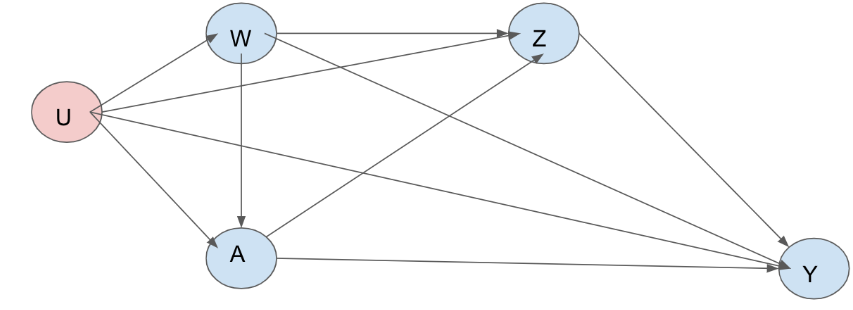
\includegraphics[width=0.5\linewidth]{./dags/dag_causal} 

}

\caption{Causal Graph for the SCM}\label{fig:fig1}
\end{figure}

\subsection{Step 2: Counterfactuals \& Causal
Parameter}\label{step-2-counterfactuals-causal-parameter}

\paragraph{Causal Parameter}\label{causal-parameter}

\[{\Psi^*}^{i}(\mathbb{P}^*)=\mathbb{E}^*[Y_i]\ \ \ i\in \{1,2,3,4\}\]
where \(i\) represent the bin of cigarettes smoked per day. \(Y_i\)
denotes the counterfactual outcome (the ten-year development of
cardiovascular disease), if possibly contrary to fact, a person's number
of cigarettes smoked per day is within \(i^{th}\) bin.

\subsection{Step 3. Specify your observed data and its link to the
causal
model}\label{step-3.-specify-your-observed-data-and-its-link-to-the-causal-model}

The dataset is adapted from Framingham Heart Study. We assume that
Gender, Age, Education, and Number of Cigarettes per Day (\(A\)) were
collected in a questionnaire at baseline. Then, BMI, Diabetes Status,
Prevalence of Stroke, Prevalence of Hypertension, Indication of Blood
Pressure Medication, Total Cholesterol Level, Blood Pressure, and Heart
Rate were all collected after the questionnaire at a doctor's office.
Our outcome, Coronary Heart Disease, is collected at a 10-year follow
up. Note that this is unlike the original study. We assume our observed
data were generated by sampling \(n\) from a system described by our
structural causal model, so we have \(n = 4211\) copies of
\(O\overset{i.i.d}\sim \mathbb{P}_O\). We place no restrictions on the
statistical model \(\mathcal{M}\), which is thereby non-parametric. BMI
was binned using guidelines from the World Health Organization. Total
Cholesterol was binned using guidelines from the National Heart, Lung
and Blood Institute (NHLBI). Table 1 below shows the counts for each
variable in each bin of the exposure, as well as a \(\chi^2\)-test of
independence.

\begin{longtable}[]{@{}lllllll@{}}
\caption{Number of Observations in Each Bin}\tabularnewline
\toprule
& Level & {[}0,1) & {[}1,10) & {[}10,19) & {[}20,70{]} &
p\tabularnewline
\midrule
\endfirsthead
\toprule
& Level & {[}0,1) & {[}1,10) & {[}10,19) & {[}20,70{]} &
p\tabularnewline
\midrule
\endhead
n & & 2089 & 471 & 380 & 1168 &\tabularnewline
diabetes (\%) & 0 & 2022 ( 96.8) & 463 ( 98.3) & 372 ( 97.9) & 1145 (
98.0) & 0.079\tabularnewline
& 1 & 67 ( 3.2) & 8 ( 1.7) & 8 ( 2.1) & 23 ( 2.0) &\tabularnewline
prevalentStroke (\%) & 0 & 2071 ( 99.1) & 469 ( 99.6) & 377 ( 99.2) &
1166 ( 99.8) & 0.095\tabularnewline
& 1 & 18 ( 0.9) & 2 ( 0.4) & 3 ( 0.8) & 2 ( 0.2) &\tabularnewline
prevalentHyp (\%) & 0 & 1337 ( 64.0) & 338 ( 71.8) & 293 ( 77.1) & 860 (
73.6) & \textless{}0.001\tabularnewline
& 1 & 752 ( 36.0) & 133 ( 28.2) & 87 ( 22.9) & 308 ( 26.4)
&\tabularnewline
age (\%) & {[}32, 42) & 363 ( 17.4) & 117 ( 24.8) & 110 ( 28.9) & 309 (
26.5) & \textless{}0.001\tabularnewline
& {[}42, 49) & 464 ( 22.2) & 137 ( 29.1) & 125 ( 32.9) & 401 ( 34.3)
&\tabularnewline
& {[}49, 56) & 527 ( 25.2) & 97 ( 20.6) & 71 ( 18.7) & 254 ( 21.7)
&\tabularnewline
& {[}56, 70{]} & 735 ( 35.2) & 120 ( 25.5) & 74 ( 19.5) & 204 ( 17.5)
&\tabularnewline
education (\%) & 1 & 915 ( 43.8) & 188 ( 39.9) & 137 ( 36.1) & 470 (
40.2) & 0.003\tabularnewline
& 2 & 574 ( 27.5) & 150 ( 31.8) & 121 ( 31.8) & 399 ( 34.2)
&\tabularnewline
& 3 & 367 ( 17.6) & 76 ( 16.1) & 71 ( 18.7) & 170 ( 14.6)
&\tabularnewline
& 4 & 233 ( 11.2) & 57 ( 12.1) & 51 ( 13.4) & 129 ( 11.0)
&\tabularnewline
BP (\%) & 0 & 1139 ( 54.5) & 267 ( 56.7) & 211 ( 55.5) & 701 ( 60.0) &
0.025\tabularnewline
& 1 & 950 ( 45.5) & 204 ( 43.3) & 169 ( 44.5) & 467 ( 40.0)
&\tabularnewline
totChol (\%) & {[}0, 200) & 386 ( 18.6) & 108 ( 23.4) & 84 ( 22.3) & 227
( 19.7) & 0.004\tabularnewline
& {[}200, 240) & 723 ( 34.9) & 151 ( 32.7) & 157 ( 41.8) & 401 ( 34.9)
&\tabularnewline
& {[}240, 600{]} & 962 ( 46.5) & 203 ( 43.9) & 135 ( 35.9) & 522 ( 45.4)
&\tabularnewline
gender (\%) & 0 & 1400 ( 67.0) & 346 ( 73.5) & 222 ( 58.4) & 386 ( 33.0)
& \textless{}0.001\tabularnewline
& 1 & 689 ( 33.0) & 125 ( 26.5) & 158 ( 41.6) & 782 ( 67.0)
&\tabularnewline
bmi (\%) & {[}0, 18.5) & 19 ( 0.9) & 13 ( 2.8) & 7 ( 1.8) & 17 ( 1.5) &
\textless{}0.001\tabularnewline
& {[}18.5, 25) & 785 ( 37.8) & 245 ( 52.2) & 225 ( 59.2) & 568 ( 48.8)
&\tabularnewline
& {[}25, 30) & 940 ( 45.3) & 170 ( 36.2) & 117 ( 30.8) & 467 ( 40.1)
&\tabularnewline
& {[}30, 56.8{]} & 333 ( 16.0) & 41 ( 8.7) & 31 ( 8.2) & 112 ( 9.6)
&\tabularnewline
heartRate (\%) & {[}0, 60) & 122 ( 5.8) & 27 ( 5.7) & 19 ( 5.0) & 28 (
2.4) & \textless{}0.001\tabularnewline
& {[}60, 143{]} & 1967 ( 94.2) & 444 ( 94.3) & 360 ( 95.0) & 1140 (
97.6) &\tabularnewline
CHD (\%) & 0 & 1784 ( 85.4) & 420 ( 89.2) & 320 ( 84.2) & 958 ( 82.0) &
0.002\tabularnewline
& 1 & 305 ( 14.6) & 51 ( 10.8) & 60 ( 15.8) & 210 ( 18.0)
&\tabularnewline
\bottomrule
\end{longtable}

\subsection{Step 4. Identifiability}\label{step-4.-identifiability}

Since we made no independence assumptions on our exogenous background
factors, we will need to make additional independence assumptions for
identifiability. For the target causal parameter in the SCM
\(\mathcal{M^*}\) to be identified from the observed data distribution,
we need to make a randomization and a positivity assumption.

\paragraph{1) Randomization Assumption:}\label{randomization-assumption}

Conditional on \(W\), the counterfactual outcome is independent of the
observed treatment: \[ Y \perp  A|W\]

\begin{figure}

{\centering 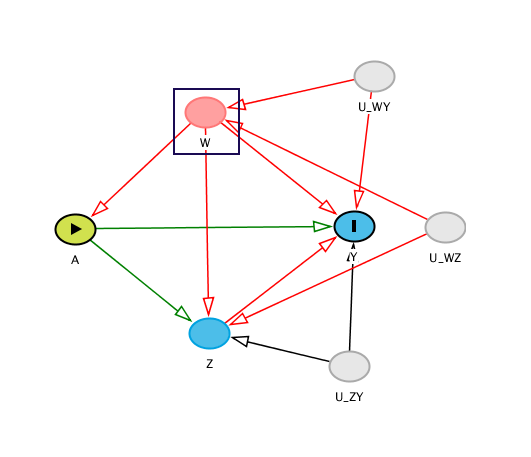
\includegraphics[width=0.5\linewidth]{./dags/augmented_dag} 

}

\caption{Causal Graph for the SCM}\label{fig:figc}
\end{figure}

\[U_A\perp U_Y,U_A\perp U_W,U_A\perp U_Z\]

In this augmented/working SCM (\(\mathcal{M^{**}}\)), the unmeasured
background factor of \(A\) (cigarettes smoked per day) is independent of
the unmeasured background factor of \(Y\) (10yr CHD), the unmeasured
background factor of \(W\) (baseline age, gender, education, diabetes,
BMI), and the unmeasured background factor of \(Z\) (prevalence of
stroke, hypertension, blood pressure, blood pressure medication, heart
rate).

Since \(W\),\(Z\), and \(Y\) include SES and biological factors that
affect human health, we aviod assuming independence between their
unmeasured background factors. Thus, we consider it is more plausible to
make the indepedence assumptions listed. We do not the mediator \(Z\) to
avoid opening a backdoor path. Under \(M^**\), the backdoor criterion
holds conditional on \(W\). Additional data on factors that affect heath
status and determinants could help with identifiability, but those
factors are not well-understood.

\paragraph{2) Positivity Assumption:}\label{positivity-assumption}

There must be a positive probability of each treatment condition within
each possible strata of \(W\). We need a positive probability of
cigarettes smoked per day for each strata of \(W\).

\[
\begin{aligned}
min_{i\in A}\mathbb{P}_0(A=i|W=w)>0\\
\text{for all}\ w \ \text{for which} 
\mathbb{P}_0(W = w) \geq 0
\end{aligned}
\] where \(i\) denote the index of a bin of \(A\).

\section{THIS NEEDS TO BE FIXED!!!!}\label{this-needs-to-be-fixed}

We are concerned about a positivity assumption violation for a bin with
high numbers of cigarettes smoked per day since certain strata of \(W\)
might not smoke at all, and binning could make particular stratas have
low probabilities of smoking certain numbers of cigarettes per day. We
can informally check for a positivity assumption violation from tables
of \(A\) given a strata of \(W\). One table from a strata of \(W\) is
shown below:

\begin{table}[ht]
\centering
\caption{Table for BMI = [18.5, 25), Gender = 0, Diabetes = 0, A = 0 }
\small
\begin{tabular}{|l|l|l|l|l|l|}
\hline
Strata & Education: 1 & Education: 2 & Education: 3 & Education: 4 & Education: NA \\ \hline
Age: [32, 42) & 26 & 60 & 32 & 12 &  1 \\ \hline
Age: [42, 49) & 40 & 42 & 41 & 18 &  0 \\ \hline
Age: [49, 56) & 43 & 52 & 42 & 17 &  5  \\ \hline
Age: [56, 70] & 75 & 41 & 36 & 16 &  2  \\ \hline
\end{tabular}
\end{table}

From the table above, we can see that we have 0 female whose BMI is in
the range {[}18.5, 25), age is in the range of {[}42, 49), education
level is missing, who does not have Diabetes, who does not smoke
cigarettes. Thus, we have a sparsity issue.

\section{NEED TO FIX ABOVE!!!!}\label{need-to-fix-above}

We also calculated the predicted probability of each bin of \(A\) (the
number of cigarettes smoked per day) given a strata of \(W\):

\begin{longtable}[]{@{}lrrrrrr@{}}
\caption{Predicted Probabilities of CHD for each Strata of
W}\tabularnewline
\toprule
& c.0.285367089748959..0.0612950549329788..0.0592083666852972.. &
c.0.427146494355085..0.0743610835769698..0.0680967575002984.. &
c.0.496890467062084..0.130851483132409..0.0894467944558553..0.221903501631759
&
c.0.508519961051581..0.114654333008947..0.0925024342753821..0.284323271665553
&
c.0.633555593922955..0.153716386674473..0.114911135918826..0.45159495956664
&
c.0.744054639002225..0.173331986730923..0.142804434050837..0.563099017937758\tabularnewline
\midrule
\endfirsthead
\toprule
& c.0.285367089748959..0.0612950549329788..0.0592083666852972.. &
c.0.427146494355085..0.0743610835769698..0.0680967575002984.. &
c.0.496890467062084..0.130851483132409..0.0894467944558553..0.221903501631759
&
c.0.508519961051581..0.114654333008947..0.0925024342753821..0.284323271665553
&
c.0.633555593922955..0.153716386674473..0.114911135918826..0.45159495956664
&
c.0.744054639002225..0.173331986730923..0.142804434050837..0.563099017937758\tabularnewline
\midrule
\endhead
i=1 & 0.2853671 & 0.4271465 & 0.4968905 & 0.5085200 & 0.6335556 &
0.7440546\tabularnewline
i=2 & 0.0612951 & 0.0743611 & 0.1308515 & 0.1146543 & 0.1537164 &
0.1733320\tabularnewline
i=3 & 0.0592084 & 0.0680968 & 0.0894468 & 0.0925024 & 0.1149111 &
0.1428044\tabularnewline
i=4 & 0.0765399 & 0.1628045 & 0.2219035 & 0.2843233 & 0.4515950 &
0.5630990\tabularnewline
\bottomrule
\end{longtable}

From the table, we can see that the probabiliy of falling into the last
bin of \(A\), which is \(\geq 20\) cigarettes smoked per day, is very
close to zero, indicating a practical violation of positivity
assumption. Theoretically, randomizing the number of cigarettes smoked
per day could help with identifiability, but it is not feasible.

\subsection{Step 5. Statistical Model and
Estimand}\label{step-5.-statistical-model-and-estimand}

The target parameter of \(\mathbb{P}_0\), which equals the causal
parameter in the augmented causal model \(\mathcal{M}^{**}\) is given by
the G-Computation formula:

\[
\begin{aligned}
\Psi_0(\mathbb{P}^i_0)&=\mathbb{E}_0[\mathbb{E}_0[Y|A= i,W=w]]\\
&= \sum_w\mathbb{E}_0[Y|A=i,W=w]*\mathbb{P}_0(W=w)
\end{aligned}
\]

\subsection{Step 6. Estimation}\label{step-6.-estimation}

\subsubsection{Conditional Mean outcome}\label{conditional-mean-outcome}

\begin{Shaded}
\begin{Highlighting}[]
\KeywordTok{library}\NormalTok{(mgcv)}
\end{Highlighting}
\end{Shaded}

\begin{verbatim}
## Loading required package: nlme
\end{verbatim}

\begin{verbatim}
## 
## Attaching package: 'nlme'
\end{verbatim}

\begin{verbatim}
## The following object is masked from 'package:dplyr':
## 
##     collapse
\end{verbatim}

\begin{verbatim}
## This is mgcv 1.8-20. For overview type 'help("mgcv-package")'.
\end{verbatim}

\begin{verbatim}
## 
## Attaching package: 'mgcv'
\end{verbatim}

\begin{verbatim}
## The following object is masked from 'package:nnet':
## 
##     multinom
\end{verbatim}

\begin{Shaded}
\begin{Highlighting}[]
\NormalTok{n_bootstrap_samples <-}\DecValTok{10}
\NormalTok{conMean_bootstrap <-}\StringTok{ }\KeywordTok{matrix}\NormalTok{(}\OtherTok{NA}\NormalTok{, }\DataTypeTok{nrow=}\NormalTok{n_bootstrap_samples,}\DataTypeTok{ncol=}\DecValTok{4}\NormalTok{)}

\ControlFlowTok{for}\NormalTok{(i }\ControlFlowTok{in} \DecValTok{1}\OperatorTok{:}\NormalTok{n_bootstrap_samples)\{}
  \KeywordTok{set.seed}\NormalTok{(i)}
\NormalTok{  fhs_binned_sample <-}\StringTok{ }\NormalTok{fhs_binned[}\KeywordTok{sample}\NormalTok{(}\DecValTok{1}\OperatorTok{:}\KeywordTok{nrow}\NormalTok{(fhs_binned),}\KeywordTok{nrow}\NormalTok{(fhs_binned),}\DataTypeTok{replace=}\OtherTok{TRUE}\NormalTok{),]}
  
\NormalTok{  intervene_on_bin <-}\StringTok{ }\ControlFlowTok{function}\NormalTok{(i)\{}
\NormalTok{  fhs_binned_i <-}\StringTok{ }\NormalTok{fhs_binned_sample}
\NormalTok{  fhs_binned_i}\OperatorTok{$}\NormalTok{cigsPerDay <-}\KeywordTok{levels}\NormalTok{(fhs_binned_sample}\OperatorTok{$}\NormalTok{cigsPerDay)[i]}
  \KeywordTok{return}\NormalTok{ (fhs_binned_i)}
\NormalTok{\}}


  
\NormalTok{## SATURED REGRESSION MODEL FOR NPMLE}
\NormalTok{glm_fit <-}\StringTok{ }\KeywordTok{glm}\NormalTok{( CHD }\OperatorTok{~}\StringTok{ }\NormalTok{cigsPerDay}\OperatorTok{*}\NormalTok{education}\OperatorTok{*}\NormalTok{age}\OperatorTok{*}\NormalTok{gender, }\DataTypeTok{data =}\NormalTok{ fhs_binned_sample, }\DataTypeTok{family =} \StringTok{"binomial"}\NormalTok{)}

\ControlFlowTok{for}\NormalTok{ (j }\ControlFlowTok{in} \DecValTok{1}\OperatorTok{:}\KeywordTok{length}\NormalTok{(}\KeywordTok{levels}\NormalTok{(fhs_binned}\OperatorTok{$}\NormalTok{cigsPerDay)))\{}
\NormalTok{  conMean_bootstrap[i,j] <-}\StringTok{ }\KeywordTok{mean}\NormalTok{(}\KeywordTok{predict}\NormalTok{(glm_fit, }\DataTypeTok{newdata=}\KeywordTok{intervene_on_bin}\NormalTok{(j), }\DataTypeTok{type=}\StringTok{'response'}\NormalTok{))}
\NormalTok{\}}
\NormalTok{\}}
\end{Highlighting}
\end{Shaded}

\begin{verbatim}
## Warning: glm.fit: fitted probabilities numerically 0 or 1 occurred

## Warning: glm.fit: fitted probabilities numerically 0 or 1 occurred

## Warning: glm.fit: fitted probabilities numerically 0 or 1 occurred

## Warning: glm.fit: fitted probabilities numerically 0 or 1 occurred

## Warning: glm.fit: fitted probabilities numerically 0 or 1 occurred

## Warning: glm.fit: fitted probabilities numerically 0 or 1 occurred

## Warning: glm.fit: fitted probabilities numerically 0 or 1 occurred

## Warning: glm.fit: fitted probabilities numerically 0 or 1 occurred

## Warning: glm.fit: fitted probabilities numerically 0 or 1 occurred

## Warning: glm.fit: fitted probabilities numerically 0 or 1 occurred
\end{verbatim}

\begin{Shaded}
\begin{Highlighting}[]
\NormalTok{average_treatment_effect <-}\StringTok{ }\KeywordTok{c}\NormalTok{()}
\NormalTok{average_treatment_effect_ci <-}\StringTok{ }\KeywordTok{matrix}\NormalTok{(}\OtherTok{NA}\NormalTok{,}\DataTypeTok{nrow=}\KeywordTok{length}\NormalTok{(}\KeywordTok{levels}\NormalTok{(fhs_binned_sample}\OperatorTok{$}\NormalTok{cigsPerDay)),}\DataTypeTok{ncol=}\DecValTok{2}\NormalTok{)}
\ControlFlowTok{for}\NormalTok{ (i }\ControlFlowTok{in} \DecValTok{1}\OperatorTok{:}\KeywordTok{length}\NormalTok{(}\KeywordTok{levels}\NormalTok{(fhs_binned_sample}\OperatorTok{$}\NormalTok{cigsPerDay)))\{}
\NormalTok{  average_treatment_effect[i] <-}\StringTok{ }\KeywordTok{colMeans}\NormalTok{(conMean_bootstrap)[i]}
\NormalTok{  average_treatment_effect_ci[i,] <-}\StringTok{ }\KeywordTok{quantile}\NormalTok{(conMean_bootstrap[,i],}\DataTypeTok{probs=}\KeywordTok{c}\NormalTok{(.}\DecValTok{025}\NormalTok{,.}\DecValTok{975}\NormalTok{))}

\NormalTok{\}}

\KeywordTok{plot}\NormalTok{(average_treatment_effect,}\DataTypeTok{ylab=}\StringTok{"Probability of CHD"}\NormalTok{,}\DataTypeTok{ylim=}\KeywordTok{c}\NormalTok{(}\DecValTok{0}\NormalTok{,.}\DecValTok{5}\NormalTok{),}
     \DataTypeTok{main =} \StringTok{"Simple Substitution"}\NormalTok{)}
\KeywordTok{points}\NormalTok{(average_treatment_effect_ci[,}\DecValTok{1}\NormalTok{],}\DataTypeTok{col=}\StringTok{'red'}\NormalTok{,}\DataTypeTok{lty=}\DecValTok{2}\NormalTok{)}
\KeywordTok{points}\NormalTok{(average_treatment_effect_ci[,}\DecValTok{2}\NormalTok{],}\DataTypeTok{col=}\StringTok{'red'}\NormalTok{,}\DataTypeTok{lty=}\DecValTok{2}\NormalTok{)}
\end{Highlighting}
\end{Shaded}

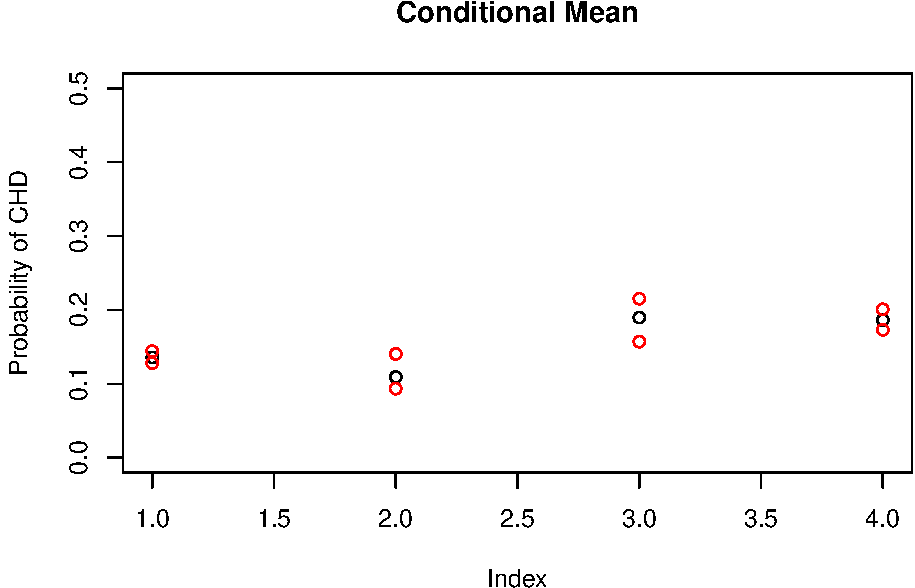
\includegraphics{framingham_files/figure-latex/unnamed-chunk-7-1.pdf}

\subsubsection{IPTW}\label{iptw}

\begin{Shaded}
\begin{Highlighting}[]
\NormalTok{n_bootstrap_samples <-}\DecValTok{10}
\NormalTok{iptw_bootstrap <-}\StringTok{ }\KeywordTok{matrix}\NormalTok{(}\OtherTok{NA}\NormalTok{, }\DataTypeTok{nrow=}\NormalTok{n_bootstrap_samples,}\DataTypeTok{ncol=}\DecValTok{4}\NormalTok{)}

\ControlFlowTok{for}\NormalTok{ (i }\ControlFlowTok{in} \DecValTok{1}\OperatorTok{:}\NormalTok{n_bootstrap_samples)\{}
  \KeywordTok{set.seed}\NormalTok{(i)}
\NormalTok{  fhs_binned_sample <-}\StringTok{ }\NormalTok{fhs_binned[}\KeywordTok{sample}\NormalTok{(}\DecValTok{1}\OperatorTok{:}\KeywordTok{nrow}\NormalTok{(fhs_binned),}\KeywordTok{nrow}\NormalTok{(fhs_binned),}\DataTypeTok{replace=}\OtherTok{TRUE}\NormalTok{),]}

\NormalTok{### BIN 1}
\NormalTok{glm_fit_iptw_bin_}\DecValTok{1}\NormalTok{ <-}\StringTok{ }\KeywordTok{glm}\NormalTok{( cigsPerDay_bin_}\DecValTok{1} \OperatorTok{~}\StringTok{   }\NormalTok{education }\OperatorTok{+}\StringTok{ }\NormalTok{age }\OperatorTok{+}\StringTok{ }\NormalTok{gender, }\DataTypeTok{data =}\NormalTok{ fhs_binned_sample, }\DataTypeTok{family =} \StringTok{"binomial"}\NormalTok{)}
\NormalTok{prob.1W <-}\StringTok{ }\KeywordTok{predict}\NormalTok{(glm_fit_iptw_bin_}\DecValTok{1}\NormalTok{, }\DataTypeTok{type=} \StringTok{"response"}\NormalTok{)}
\NormalTok{wt_}\DecValTok{1}\NormalTok{<-}\StringTok{ }\DecValTok{1}\OperatorTok{/}\NormalTok{prob.1W}
\KeywordTok{summary}\NormalTok{(wt_}\DecValTok{1}\NormalTok{)}
\NormalTok{IPTW_bin_}\DecValTok{1}\NormalTok{<-}\StringTok{ }\KeywordTok{mean}\NormalTok{( wt_}\DecValTok{1}\OperatorTok{*}\KeywordTok{as.numeric}\NormalTok{(fhs_binned_sample}\OperatorTok{$}\NormalTok{cigsPerDay_bin_}\DecValTok{1}\OperatorTok{==}\DecValTok{1}\NormalTok{)}\OperatorTok{*}\KeywordTok{as.numeric}\NormalTok{(fhs_binned_sample}\OperatorTok{$}\NormalTok{CHD}\OperatorTok{==}\DecValTok{1}\NormalTok{))}


\NormalTok{### BIN 2}
\NormalTok{glm_fit_iptw_bin_}\DecValTok{2}\NormalTok{ <-}\StringTok{ }\KeywordTok{glm}\NormalTok{( cigsPerDay_bin_}\DecValTok{2} \OperatorTok{~}\StringTok{   }\NormalTok{education }\OperatorTok{+}\StringTok{ }\NormalTok{age }\OperatorTok{+}\StringTok{ }\NormalTok{gender, }\DataTypeTok{data =}\NormalTok{ fhs_binned_sample, }\DataTypeTok{family =} \StringTok{"binomial"}\NormalTok{)}
\NormalTok{prob.1W <-}\StringTok{ }\KeywordTok{predict}\NormalTok{(glm_fit_iptw_bin_}\DecValTok{2}\NormalTok{, }\DataTypeTok{type=} \StringTok{"response"}\NormalTok{)}
\NormalTok{wt_}\DecValTok{2}\NormalTok{<-}\StringTok{ }\DecValTok{1}\OperatorTok{/}\NormalTok{prob.1W}
\KeywordTok{summary}\NormalTok{(wt_}\DecValTok{2}\NormalTok{)}
\NormalTok{IPTW_bin_}\DecValTok{2}\NormalTok{<-}\StringTok{ }\KeywordTok{mean}\NormalTok{( wt_}\DecValTok{2}\OperatorTok{*}\KeywordTok{as.numeric}\NormalTok{(fhs_binned_sample}\OperatorTok{$}\NormalTok{cigsPerDay_bin_}\DecValTok{2}\OperatorTok{==}\DecValTok{1}\NormalTok{)}\OperatorTok{*}\KeywordTok{as.numeric}\NormalTok{(fhs_binned_sample}\OperatorTok{$}\NormalTok{CHD}\OperatorTok{==}\DecValTok{1}\NormalTok{))}

\NormalTok{### BIN 3}
\NormalTok{glm_fit_iptw_bin_}\DecValTok{3}\NormalTok{ <-}\StringTok{ }\KeywordTok{glm}\NormalTok{( cigsPerDay_bin_}\DecValTok{3} \OperatorTok{~}\StringTok{  }\NormalTok{education }\OperatorTok{+}\StringTok{ }\NormalTok{age }\OperatorTok{+}\StringTok{ }\NormalTok{gender, }\DataTypeTok{data =}\NormalTok{ fhs_binned_sample, }\DataTypeTok{family =} \StringTok{"binomial"}\NormalTok{)}
\NormalTok{prob.1W <-}\StringTok{ }\KeywordTok{predict}\NormalTok{(glm_fit_iptw_bin_}\DecValTok{3}\NormalTok{, }\DataTypeTok{type=} \StringTok{"response"}\NormalTok{)}
\NormalTok{wt_}\DecValTok{3}\NormalTok{<-}\StringTok{ }\DecValTok{1}\OperatorTok{/}\NormalTok{prob.1W}
\KeywordTok{summary}\NormalTok{(wt_}\DecValTok{3}\NormalTok{)}
\NormalTok{IPTW_bin_}\DecValTok{3}\NormalTok{<-}\StringTok{ }\KeywordTok{mean}\NormalTok{( wt_}\DecValTok{3}\OperatorTok{*}\KeywordTok{as.numeric}\NormalTok{(fhs_binned_sample}\OperatorTok{$}\NormalTok{cigsPerDay_bin_}\DecValTok{3}\OperatorTok{==}\DecValTok{1}\NormalTok{)}\OperatorTok{*}\KeywordTok{as.numeric}\NormalTok{(fhs_binned_sample}\OperatorTok{$}\NormalTok{CHD}\OperatorTok{==}\DecValTok{1}\NormalTok{))}


\NormalTok{### BIN 4}
\NormalTok{glm_fit_iptw_bin_}\DecValTok{4}\NormalTok{ <-}\StringTok{ }\KeywordTok{glm}\NormalTok{( cigsPerDay_bin_}\DecValTok{4} \OperatorTok{~}\StringTok{  }\NormalTok{education }\OperatorTok{+}\StringTok{ }\NormalTok{age }\OperatorTok{+}\StringTok{ }\NormalTok{gender, }\DataTypeTok{data =}\NormalTok{ fhs_binned_sample, }\DataTypeTok{family =} \StringTok{"binomial"}\NormalTok{)}
\NormalTok{prob.1W <-}\StringTok{ }\KeywordTok{predict}\NormalTok{(glm_fit_iptw_bin_}\DecValTok{4}\NormalTok{, }\DataTypeTok{type=} \StringTok{"response"}\NormalTok{)}
\NormalTok{wt_}\DecValTok{4}\NormalTok{<-}\StringTok{ }\DecValTok{1}\OperatorTok{/}\NormalTok{prob.1W}
\KeywordTok{summary}\NormalTok{(wt_}\DecValTok{4}\NormalTok{)}
\NormalTok{IPTW_bin_}\DecValTok{4}\NormalTok{<-}\StringTok{ }\KeywordTok{mean}\NormalTok{( wt_}\DecValTok{4}\OperatorTok{*}\KeywordTok{as.numeric}\NormalTok{(fhs_binned_sample}\OperatorTok{$}\NormalTok{cigsPerDay_bin_}\DecValTok{4}\OperatorTok{==}\DecValTok{1}\NormalTok{)}\OperatorTok{*}\KeywordTok{as.numeric}\NormalTok{(fhs_binned_sample}\OperatorTok{$}\NormalTok{CHD}\OperatorTok{==}\DecValTok{1}\NormalTok{))}

\NormalTok{iptw_bootstrap[i,] =}\StringTok{ }\KeywordTok{c}\NormalTok{(IPTW_bin_}\DecValTok{1}\NormalTok{, IPTW_bin_}\DecValTok{2}\NormalTok{, IPTW_bin_}\DecValTok{3}\NormalTok{, IPTW_bin_}\DecValTok{4}\NormalTok{)}
\NormalTok{\}}

\NormalTok{average_treatment_effect <-}\StringTok{ }\KeywordTok{c}\NormalTok{()}
\NormalTok{average_treatment_effect_ci <-}\StringTok{ }\KeywordTok{matrix}\NormalTok{(}\OtherTok{NA}\NormalTok{,}\DataTypeTok{nrow=}\KeywordTok{length}\NormalTok{(}\KeywordTok{levels}\NormalTok{(fhs_binned_sample}\OperatorTok{$}\NormalTok{cigsPerDay)),}\DataTypeTok{ncol=}\DecValTok{2}\NormalTok{)}
\ControlFlowTok{for}\NormalTok{ (i }\ControlFlowTok{in} \DecValTok{1}\OperatorTok{:}\KeywordTok{length}\NormalTok{(}\KeywordTok{levels}\NormalTok{(fhs_binned_sample}\OperatorTok{$}\NormalTok{cigsPerDay)))\{}
\NormalTok{  average_treatment_effect[i] <-}\StringTok{ }\KeywordTok{colMeans}\NormalTok{(iptw_bootstrap)[i]}
\NormalTok{  average_treatment_effect_ci[i,] <-}\StringTok{ }\KeywordTok{quantile}\NormalTok{(iptw_bootstrap[,i],}\DataTypeTok{probs=}\KeywordTok{c}\NormalTok{(.}\DecValTok{025}\NormalTok{,.}\DecValTok{975}\NormalTok{))}

\NormalTok{\}}

\KeywordTok{plot}\NormalTok{(average_treatment_effect,}\DataTypeTok{ylab=}\StringTok{"Probability of CHD"}\NormalTok{,}\DataTypeTok{ylim=}\KeywordTok{c}\NormalTok{(}\DecValTok{0}\NormalTok{,.}\DecValTok{5}\NormalTok{),}
     \DataTypeTok{main =} \StringTok{"IPTW"}\NormalTok{)}
\KeywordTok{points}\NormalTok{(average_treatment_effect_ci[,}\DecValTok{1}\NormalTok{],}\DataTypeTok{col=}\StringTok{'red'}\NormalTok{,}\DataTypeTok{lty=}\DecValTok{2}\NormalTok{)}
\KeywordTok{points}\NormalTok{(average_treatment_effect_ci[,}\DecValTok{2}\NormalTok{],}\DataTypeTok{col=}\StringTok{'red'}\NormalTok{,}\DataTypeTok{lty=}\DecValTok{2}\NormalTok{)}
\end{Highlighting}
\end{Shaded}

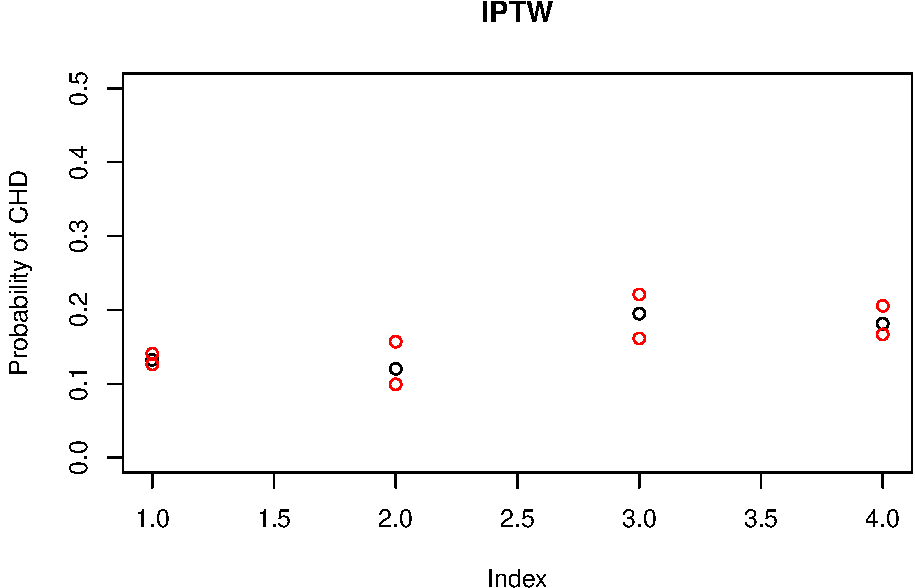
\includegraphics{framingham_files/figure-latex/unnamed-chunk-8-1.pdf}

\begin{Shaded}
\begin{Highlighting}[]
\KeywordTok{hist}\NormalTok{(wt_}\DecValTok{1}\NormalTok{,}\DataTypeTok{xlab=}\StringTok{"Weights of bin 1"}\NormalTok{)}
\end{Highlighting}
\end{Shaded}

\includegraphics{framingham_files/figure-latex/unnamed-chunk-8-2.pdf}

\begin{Shaded}
\begin{Highlighting}[]
\KeywordTok{hist}\NormalTok{(wt_}\DecValTok{2}\NormalTok{,}\DataTypeTok{xlab=}\StringTok{"Weights of bin 2"}\NormalTok{)}
\end{Highlighting}
\end{Shaded}

\includegraphics{framingham_files/figure-latex/unnamed-chunk-8-3.pdf}

\begin{Shaded}
\begin{Highlighting}[]
\KeywordTok{hist}\NormalTok{(wt_}\DecValTok{3}\NormalTok{,}\DataTypeTok{xlab=}\StringTok{"Weights of bin 3"}\NormalTok{)}
\end{Highlighting}
\end{Shaded}

\includegraphics{framingham_files/figure-latex/unnamed-chunk-8-4.pdf}

\begin{Shaded}
\begin{Highlighting}[]
\KeywordTok{hist}\NormalTok{(wt_}\DecValTok{4}\NormalTok{,}\DataTypeTok{xlab=}\StringTok{"Weights of bin 4"}\NormalTok{)}
\end{Highlighting}
\end{Shaded}

\includegraphics{framingham_files/figure-latex/unnamed-chunk-8-5.pdf}

\subsubsection{Superlearner/TMLE}\label{superlearnertmle}

\begin{Shaded}
\begin{Highlighting}[]
\KeywordTok{library}\NormalTok{(}\StringTok{'SuperLearner'}\NormalTok{)}
\end{Highlighting}
\end{Shaded}

\begin{verbatim}
## Warning: package 'SuperLearner' was built under R version 3.4.4
\end{verbatim}

\begin{verbatim}
## Loading required package: nnls
\end{verbatim}

\begin{verbatim}
## Super Learner
\end{verbatim}

\begin{verbatim}
## Version: 2.0-24
\end{verbatim}

\begin{verbatim}
## Package created on 2018-08-10
\end{verbatim}

\begin{Shaded}
\begin{Highlighting}[]
\NormalTok{SL.library<-}\StringTok{ }\KeywordTok{c}\NormalTok{(}\StringTok{"SL.glmnet"}\NormalTok{,}\StringTok{"SL.randomForest"}\NormalTok{,}\StringTok{"SL.nnet"}\NormalTok{,}\StringTok{"SL.earth"}\NormalTok{,}\StringTok{"SL.bayesglm"}\NormalTok{)}

\NormalTok{n_bootstrap_samples <-}\DecValTok{1}
\NormalTok{tmle_bootstrap_bin_}\DecValTok{1}\NormalTok{ <-}\StringTok{ }\KeywordTok{c}\NormalTok{()}

\ControlFlowTok{for}\NormalTok{ (i }\ControlFlowTok{in} \DecValTok{1}\OperatorTok{:}\NormalTok{n_bootstrap_samples)\{}
  \KeywordTok{set.seed}\NormalTok{(i)}
\NormalTok{  ### BIN1 TMLE}
\NormalTok{  fhs_binned_sample <-}\StringTok{ }\NormalTok{fhs_binned[}\KeywordTok{sample}\NormalTok{(}\DecValTok{1}\OperatorTok{:}\KeywordTok{nrow}\NormalTok{(fhs_binned),}\KeywordTok{nrow}\NormalTok{(fhs_binned),}\DataTypeTok{replace=}\OtherTok{TRUE}\NormalTok{),]}
  
\NormalTok{  X_minus_bin_}\DecValTok{1}\NormalTok{<-}\StringTok{ }\KeywordTok{subset}\NormalTok{(fhs_binned_sample, }\DataTypeTok{select=} \KeywordTok{c}\NormalTok{(}\StringTok{"cigsPerDay_bin_1"}\NormalTok{, }\StringTok{"education"}\NormalTok{, }\StringTok{"age"}\NormalTok{,}\StringTok{"gender"}\NormalTok{) )}
\NormalTok{  X_minus_bin_}\DecValTok{1}\OperatorTok{$}\NormalTok{age <-}\StringTok{ }\KeywordTok{as.numeric}\NormalTok{(X_minus_bin_}\DecValTok{1}\OperatorTok{$}\NormalTok{age)}
\NormalTok{  X_minus_bin_1_all_bin_}\DecValTok{1}\NormalTok{ <-}\StringTok{ }\NormalTok{X_minus_bin_}\DecValTok{1}
\NormalTok{  X_minus_bin_1_all_bin_}\DecValTok{1}\OperatorTok{$}\NormalTok{cigsPerDay_bin_}\DecValTok{1}\NormalTok{ <-}\StringTok{ }\DecValTok{1}
  
\NormalTok{  ##CONVERT FACTORS TO NUMERIC FOR SUPERLEARNER}
  
  
\NormalTok{  SL.outcome<-}\StringTok{ }\KeywordTok{SuperLearner}\NormalTok{(}\DataTypeTok{Y=}\KeywordTok{as.numeric}\NormalTok{(fhs_binned_sample}\OperatorTok{$}\NormalTok{CHD}\OperatorTok{==}\DecValTok{1}\NormalTok{), }\DataTypeTok{X=}\NormalTok{X_minus_bin_}\DecValTok{1}\NormalTok{, }\DataTypeTok{SL.library=}\NormalTok{SL.library, }\DataTypeTok{family=}\StringTok{"binomial"}\NormalTok{)}
  
  
\NormalTok{  expY.givenA1 <-}\StringTok{  }\KeywordTok{predict}\NormalTok{(SL.outcome, }\DataTypeTok{newdata=}\NormalTok{X_minus_bin_1_all_bin_}\DecValTok{1}\NormalTok{)}\OperatorTok{$}\NormalTok{pred}
\NormalTok{  SL.exposure<-}\StringTok{ }\KeywordTok{SuperLearner}\NormalTok{(}\DataTypeTok{Y=}\KeywordTok{as.numeric}\NormalTok{(fhs_binned}\OperatorTok{$}\NormalTok{cigsPerDay_bin_}\DecValTok{1}\OperatorTok{==}\DecValTok{1}\NormalTok{), }\DataTypeTok{X=}\KeywordTok{subset}\NormalTok{(X_minus_bin_}\DecValTok{1}\NormalTok{, }\DataTypeTok{select=} \OperatorTok{-}\KeywordTok{c}\NormalTok{(cigsPerDay_bin_}\DecValTok{1}\NormalTok{)),}\DataTypeTok{SL.library=}\NormalTok{SL.library, }\DataTypeTok{family=}\StringTok{"binomial"}\NormalTok{)}
\NormalTok{  probA1.givenW<-}\StringTok{ }\NormalTok{SL.exposure}\OperatorTok{$}\NormalTok{SL.predict}
\NormalTok{  H.AW<-}\StringTok{ }\KeywordTok{as.numeric}\NormalTok{(fhs_binned}\OperatorTok{$}\NormalTok{cigsPerDay_bin_}\DecValTok{1}\OperatorTok{==}\DecValTok{1}\NormalTok{)}\OperatorTok{/}\NormalTok{probA1.givenW}
\NormalTok{  logitUpdate<-}\StringTok{ }\KeywordTok{glm}\NormalTok{(fhs_binned}\OperatorTok{$}\NormalTok{CHD }\OperatorTok{~}\StringTok{ }\OperatorTok{-}\DecValTok{1} \OperatorTok{+}\KeywordTok{offset}\NormalTok{(}\KeywordTok{qlogis}\NormalTok{(expY.givenA1)) }\OperatorTok{+}\StringTok{ }\NormalTok{H.AW, }\DataTypeTok{family=}\StringTok{'binomial'}\NormalTok{)}
\NormalTok{  epsilon<-}\StringTok{ }\NormalTok{logitUpdate}\OperatorTok{$}\NormalTok{coef}
\NormalTok{  expY.givenAW.star<-}\StringTok{ }\KeywordTok{plogis}\NormalTok{(}\KeywordTok{qlogis}\NormalTok{(expY.givenA1)}\OperatorTok{+}\StringTok{ }\NormalTok{epsilon}\OperatorTok{*}\NormalTok{H.AW)}
\NormalTok{  PsiHat.TMLE_bin_}\DecValTok{1}\NormalTok{<-}\StringTok{ }\KeywordTok{mean}\NormalTok{(expY.givenAW.star)}\CommentTok{#- expY.given0W.star)}
\NormalTok{  tmle_bootstrap_bin_}\DecValTok{1}\NormalTok{[i] <-}\StringTok{ }\NormalTok{PsiHat.TMLE_bin_}\DecValTok{1}
\NormalTok{\}}
\end{Highlighting}
\end{Shaded}

\begin{verbatim}
## Loading required package: arm
\end{verbatim}

\begin{verbatim}
## Warning: package 'arm' was built under R version 3.4.4
\end{verbatim}

\begin{verbatim}
## Loading required package: MASS
\end{verbatim}

\begin{verbatim}
## 
## Attaching package: 'MASS'
\end{verbatim}

\begin{verbatim}
## The following object is masked from 'package:dplyr':
## 
##     select
\end{verbatim}

\begin{verbatim}
## Loading required package: Matrix
\end{verbatim}

\begin{verbatim}
## Loading required package: lme4
\end{verbatim}

\begin{verbatim}
## Warning: package 'lme4' was built under R version 3.4.4
\end{verbatim}

\begin{verbatim}
## 
## Attaching package: 'lme4'
\end{verbatim}

\begin{verbatim}
## The following object is masked from 'package:nlme':
## 
##     lmList
\end{verbatim}

\begin{verbatim}
## 
## arm (Version 1.10-1, built: 2018-4-12)
\end{verbatim}

\begin{verbatim}
## Working directory is /Users/gcgibson/causal_project/finalproj
\end{verbatim}

\begin{verbatim}
## Loading required package: glmnet
\end{verbatim}

\begin{verbatim}
## Loading required package: foreach
\end{verbatim}

\begin{verbatim}
## Loaded glmnet 2.0-12
\end{verbatim}

\begin{verbatim}
## Loading required package: randomForest
\end{verbatim}

\begin{verbatim}
## Warning: package 'randomForest' was built under R version 3.4.4
\end{verbatim}

\begin{verbatim}
## randomForest 4.6-14
\end{verbatim}

\begin{verbatim}
## Type rfNews() to see new features/changes/bug fixes.
\end{verbatim}

\begin{verbatim}
## 
## Attaching package: 'randomForest'
\end{verbatim}

\begin{verbatim}
## The following object is masked from 'package:dplyr':
## 
##     combine
\end{verbatim}

\begin{verbatim}
## Loading required package: earth
\end{verbatim}

\begin{verbatim}
## Warning: package 'earth' was built under R version 3.4.4
\end{verbatim}

\begin{verbatim}
## Loading required package: plotmo
\end{verbatim}

\begin{verbatim}
## Warning: package 'plotmo' was built under R version 3.4.4
\end{verbatim}

\begin{verbatim}
## Loading required package: plotrix
\end{verbatim}

\begin{verbatim}
## 
## Attaching package: 'plotrix'
\end{verbatim}

\begin{verbatim}
## The following object is masked from 'package:arm':
## 
##     rescale
\end{verbatim}

\begin{verbatim}
## Loading required package: TeachingDemos
\end{verbatim}

\begin{Shaded}
\begin{Highlighting}[]
\NormalTok{  #### BIN 2 TMLE}

\NormalTok{tmle_bootstrap_bin_}\DecValTok{2}\NormalTok{ <-}\StringTok{ }\KeywordTok{c}\NormalTok{()}
\ControlFlowTok{for}\NormalTok{ (i }\ControlFlowTok{in} \DecValTok{1}\OperatorTok{:}\NormalTok{n_bootstrap_samples)\{}
  \KeywordTok{set.seed}\NormalTok{(i)}
\NormalTok{  X_minus_bin_}\DecValTok{2}\NormalTok{<-}\StringTok{ }\KeywordTok{subset}\NormalTok{(fhs_binned_sample, }\DataTypeTok{select=} \KeywordTok{c}\NormalTok{(}\StringTok{"cigsPerDay_bin_2"}\NormalTok{, }\StringTok{"education"}\NormalTok{, }\StringTok{"age"}\NormalTok{,}\StringTok{"gender"}\NormalTok{) )}
\NormalTok{  X_minus_bin_}\DecValTok{2}\OperatorTok{$}\NormalTok{age <-}\StringTok{ }\KeywordTok{as.numeric}\NormalTok{(X_minus_bin_}\DecValTok{2}\OperatorTok{$}\NormalTok{age)}
\NormalTok{  X_minus_bin_2_all_bin_}\DecValTok{2}\NormalTok{ <-}\StringTok{ }\NormalTok{X_minus_bin_}\DecValTok{2}
\NormalTok{  X_minus_bin_2_all_bin_}\DecValTok{2}\OperatorTok{$}\NormalTok{cigsPerDay_bin_}\DecValTok{2}\NormalTok{ <-}\StringTok{ }\DecValTok{1}
  
\NormalTok{  SL.outcome<-}\StringTok{ }\KeywordTok{SuperLearner}\NormalTok{(}\DataTypeTok{Y=}\KeywordTok{as.numeric}\NormalTok{(fhs_binned_sample}\OperatorTok{$}\NormalTok{CHD}\OperatorTok{==}\DecValTok{1}\NormalTok{), }\DataTypeTok{X=}\NormalTok{X_minus_bin_}\DecValTok{2}\NormalTok{, }\DataTypeTok{SL.library=}\NormalTok{SL.library, }\DataTypeTok{family=}\StringTok{"binomial"}\NormalTok{)}
\NormalTok{  expY.givenA1 <-}\StringTok{  }\KeywordTok{predict}\NormalTok{(SL.outcome, }\DataTypeTok{newdata=}\NormalTok{X_minus_bin_2_all_bin_}\DecValTok{2}\NormalTok{)}\OperatorTok{$}\NormalTok{pred}
\NormalTok{  SL.exposure<-}\StringTok{ }\KeywordTok{SuperLearner}\NormalTok{(}\DataTypeTok{Y=}\KeywordTok{as.numeric}\NormalTok{(fhs_binned}\OperatorTok{$}\NormalTok{cigsPerDay_bin_}\DecValTok{2}\OperatorTok{==}\DecValTok{1}\NormalTok{), }\DataTypeTok{X=}\KeywordTok{subset}\NormalTok{(X_minus_bin_}\DecValTok{2}\NormalTok{, }\DataTypeTok{select=} \OperatorTok{-}\KeywordTok{c}\NormalTok{(cigsPerDay_bin_}\DecValTok{2}\NormalTok{)),}\DataTypeTok{SL.library=}\NormalTok{SL.library, }\DataTypeTok{family=}\StringTok{"binomial"}\NormalTok{)}
\NormalTok{  probA1.givenW<-}\StringTok{ }\NormalTok{SL.exposure}\OperatorTok{$}\NormalTok{SL.predict}
\NormalTok{  H.AW<-}\StringTok{ }\KeywordTok{as.numeric}\NormalTok{(fhs_binned}\OperatorTok{$}\NormalTok{cigsPerDay_bin_}\DecValTok{2}\OperatorTok{==}\DecValTok{1}\NormalTok{)}\OperatorTok{/}\NormalTok{probA1.givenW}
\NormalTok{  logitUpdate<-}\StringTok{ }\KeywordTok{glm}\NormalTok{(fhs_binned}\OperatorTok{$}\NormalTok{CHD }\OperatorTok{~}\StringTok{ }\OperatorTok{-}\DecValTok{1} \OperatorTok{+}\KeywordTok{offset}\NormalTok{(}\KeywordTok{qlogis}\NormalTok{(expY.givenA1)) }\OperatorTok{+}\StringTok{ }\NormalTok{H.AW, }\DataTypeTok{family=}\StringTok{'binomial'}\NormalTok{)}
\NormalTok{  epsilon<-}\StringTok{ }\NormalTok{logitUpdate}\OperatorTok{$}\NormalTok{coef}
\NormalTok{  expY.givenAW.star<-}\StringTok{ }\KeywordTok{plogis}\NormalTok{(}\KeywordTok{qlogis}\NormalTok{(expY.givenA1)}\OperatorTok{+}\StringTok{ }\NormalTok{epsilon}\OperatorTok{*}\NormalTok{H.AW)}
\NormalTok{  PsiHat.TMLE_bin_}\DecValTok{2}\NormalTok{<-}\StringTok{ }\KeywordTok{mean}\NormalTok{(expY.givenAW.star)}\CommentTok{#- expY.given0W.star)}
\NormalTok{  tmle_bootstrap_bin_}\DecValTok{2}\NormalTok{[i] <-}\StringTok{ }\NormalTok{PsiHat.TMLE_bin_}\DecValTok{2}
\NormalTok{\}}
\end{Highlighting}
\end{Shaded}

\begin{Shaded}
\begin{Highlighting}[]
\NormalTok{tmle_bootstrap_bin_}\DecValTok{3}\NormalTok{ <-}\StringTok{ }\KeywordTok{c}\NormalTok{()}

\ControlFlowTok{for}\NormalTok{ (i }\ControlFlowTok{in} \DecValTok{1}\OperatorTok{:}\NormalTok{n_bootstrap_samples)\{}
\NormalTok{  #### BIN 3 TMLE }
  
\NormalTok{  X_minus_bin_}\DecValTok{3}\NormalTok{<-}\StringTok{ }\KeywordTok{subset}\NormalTok{(fhs_binned_sample, }\DataTypeTok{select=} \KeywordTok{c}\NormalTok{(}\StringTok{"cigsPerDay_bin_3"}\NormalTok{, }\StringTok{"education"}\NormalTok{, }\StringTok{"age"}\NormalTok{,}\StringTok{"gender"}\NormalTok{) )}
\NormalTok{  X_minus_bin_}\DecValTok{3}\OperatorTok{$}\NormalTok{age <-}\StringTok{ }\KeywordTok{as.numeric}\NormalTok{(X_minus_bin_}\DecValTok{3}\OperatorTok{$}\NormalTok{age)}
  
\NormalTok{  X_minus_bin_3_all_bin_}\DecValTok{3}\NormalTok{ <-}\StringTok{ }\NormalTok{X_minus_bin_}\DecValTok{3}
\NormalTok{  X_minus_bin_3_all_bin_}\DecValTok{3}\OperatorTok{$}\NormalTok{cigsPerDay_bin_}\DecValTok{3}\NormalTok{ <-}\StringTok{ }\DecValTok{1}
\NormalTok{  SL.outcome<-}\StringTok{ }\KeywordTok{SuperLearner}\NormalTok{(}\DataTypeTok{Y=}\KeywordTok{as.numeric}\NormalTok{(fhs_binned_sample}\OperatorTok{$}\NormalTok{CHD}\OperatorTok{==}\DecValTok{1}\NormalTok{), }\DataTypeTok{X=}\NormalTok{X_minus_bin_}\DecValTok{3}\NormalTok{, }\DataTypeTok{SL.library=}\NormalTok{SL.library, }\DataTypeTok{family=}\StringTok{"binomial"}\NormalTok{)}
\NormalTok{  expY.givenA1 <-}\StringTok{  }\KeywordTok{predict}\NormalTok{(SL.outcome, }\DataTypeTok{newdata=}\NormalTok{X_minus_bin_3_all_bin_}\DecValTok{3}\NormalTok{)}\OperatorTok{$}\NormalTok{pred}
\NormalTok{  SL.exposure<-}\StringTok{ }\KeywordTok{SuperLearner}\NormalTok{(}\DataTypeTok{Y=}\KeywordTok{as.numeric}\NormalTok{(fhs_binned}\OperatorTok{$}\NormalTok{cigsPerDay_bin_}\DecValTok{3}\OperatorTok{==}\DecValTok{1}\NormalTok{), }\DataTypeTok{X=}\KeywordTok{subset}\NormalTok{(X_minus_bin_}\DecValTok{3}\NormalTok{, }\DataTypeTok{select=} \OperatorTok{-}\KeywordTok{c}\NormalTok{(cigsPerDay_bin_}\DecValTok{3}\NormalTok{)),}\DataTypeTok{SL.library=}\NormalTok{SL.library, }\DataTypeTok{family=}\StringTok{"binomial"}\NormalTok{)}
\NormalTok{  probA1.givenW<-}\StringTok{ }\NormalTok{SL.exposure}\OperatorTok{$}\NormalTok{SL.predict}
\NormalTok{  H.AW<-}\StringTok{ }\KeywordTok{as.numeric}\NormalTok{(fhs_binned}\OperatorTok{$}\NormalTok{cigsPerDay_bin_}\DecValTok{3}\OperatorTok{==}\DecValTok{1}\NormalTok{)}\OperatorTok{/}\NormalTok{probA1.givenW}
\NormalTok{  logitUpdate<-}\StringTok{ }\KeywordTok{glm}\NormalTok{(fhs_binned}\OperatorTok{$}\NormalTok{CHD }\OperatorTok{~}\StringTok{ }\OperatorTok{-}\DecValTok{1} \OperatorTok{+}\KeywordTok{offset}\NormalTok{(}\KeywordTok{qlogis}\NormalTok{(expY.givenA1)) }\OperatorTok{+}\StringTok{ }\NormalTok{H.AW, }\DataTypeTok{family=}\StringTok{'binomial'}\NormalTok{)}
\NormalTok{  epsilon<-}\StringTok{ }\NormalTok{logitUpdate}\OperatorTok{$}\NormalTok{coef}
\NormalTok{  expY.givenAW.star<-}\StringTok{ }\KeywordTok{plogis}\NormalTok{(}\KeywordTok{qlogis}\NormalTok{(expY.givenA1)}\OperatorTok{+}\StringTok{ }\NormalTok{epsilon}\OperatorTok{*}\NormalTok{H.AW)}
\NormalTok{  PsiHat.TMLE_bin_}\DecValTok{3}\NormalTok{ <-}\StringTok{ }\KeywordTok{mean}\NormalTok{(expY.givenAW.star)}
\NormalTok{  tmle_bootstrap_bin_}\DecValTok{3}\NormalTok{[i] <-}\StringTok{ }\NormalTok{PsiHat.TMLE_bin_}\DecValTok{3}
\NormalTok{\}}
\end{Highlighting}
\end{Shaded}

\begin{Shaded}
\begin{Highlighting}[]
\NormalTok{  #### BIN 4  TMLE }
\NormalTok{tmle_bootstrap_bin_}\DecValTok{4}\NormalTok{ <-}\StringTok{ }\KeywordTok{c}\NormalTok{()}
\ControlFlowTok{for}\NormalTok{ (i }\ControlFlowTok{in} \DecValTok{1}\OperatorTok{:}\NormalTok{n_bootstrap_samples)\{}

\NormalTok{  X_minus_bin_}\DecValTok{4}\NormalTok{<-}\StringTok{ }\KeywordTok{subset}\NormalTok{(fhs_binned_sample, }\DataTypeTok{select=} \KeywordTok{c}\NormalTok{(}\StringTok{"cigsPerDay_bin_4"}\NormalTok{, }\StringTok{"education"}\NormalTok{, }\StringTok{"age"}\NormalTok{,}\StringTok{"gender"}\NormalTok{) )}
\NormalTok{  X_minus_bin_}\DecValTok{4}\OperatorTok{$}\NormalTok{age <-}\StringTok{ }\KeywordTok{as.numeric}\NormalTok{(X_minus_bin_}\DecValTok{4}\OperatorTok{$}\NormalTok{age)}
  
\NormalTok{  X_minus_bin_4_all_bin_}\DecValTok{4}\NormalTok{ <-}\StringTok{ }\NormalTok{X_minus_bin_}\DecValTok{4}
\NormalTok{  X_minus_bin_4_all_bin_}\DecValTok{4}\OperatorTok{$}\NormalTok{cigsPerDay_bin_}\DecValTok{4}\NormalTok{ <-}\StringTok{ }\DecValTok{1}
\NormalTok{  SL.outcome<-}\StringTok{ }\KeywordTok{SuperLearner}\NormalTok{(}\DataTypeTok{Y=}\KeywordTok{as.numeric}\NormalTok{(fhs_binned_sample}\OperatorTok{$}\NormalTok{CHD}\OperatorTok{==}\DecValTok{1}\NormalTok{), }\DataTypeTok{X=}\NormalTok{X_minus_bin_}\DecValTok{4}\NormalTok{, }\DataTypeTok{SL.library=}\NormalTok{SL.library, }\DataTypeTok{family=}\StringTok{"binomial"}\NormalTok{)}
\NormalTok{  expY.givenA1 <-}\StringTok{  }\KeywordTok{predict}\NormalTok{(SL.outcome, }\DataTypeTok{newdata=}\NormalTok{X_minus_bin_4_all_bin_}\DecValTok{4}\NormalTok{)}\OperatorTok{$}\NormalTok{pred}
\NormalTok{  SL.exposure<-}\StringTok{ }\KeywordTok{SuperLearner}\NormalTok{(}\DataTypeTok{Y=}\KeywordTok{as.numeric}\NormalTok{(fhs_binned}\OperatorTok{$}\NormalTok{cigsPerDay_bin_}\DecValTok{4}\OperatorTok{==}\DecValTok{1}\NormalTok{), }\DataTypeTok{X=}\KeywordTok{subset}\NormalTok{(X_minus_bin_}\DecValTok{4}\NormalTok{, }\DataTypeTok{select=} \OperatorTok{-}\KeywordTok{c}\NormalTok{(cigsPerDay_bin_}\DecValTok{4}\NormalTok{)),}\DataTypeTok{SL.library=}\NormalTok{SL.library, }\DataTypeTok{family=}\StringTok{"binomial"}\NormalTok{)}
\NormalTok{  probA1.givenW<-}\StringTok{ }\NormalTok{SL.exposure}\OperatorTok{$}\NormalTok{SL.predict}
\NormalTok{  H.AW<-}\StringTok{ }\KeywordTok{as.numeric}\NormalTok{(fhs_binned}\OperatorTok{$}\NormalTok{cigsPerDay_bin_}\DecValTok{4}\OperatorTok{==}\DecValTok{1}\NormalTok{)}\OperatorTok{/}\NormalTok{probA1.givenW}
\NormalTok{  logitUpdate<-}\StringTok{ }\KeywordTok{glm}\NormalTok{(fhs_binned}\OperatorTok{$}\NormalTok{CHD }\OperatorTok{~}\StringTok{ }\OperatorTok{-}\DecValTok{1} \OperatorTok{+}\KeywordTok{offset}\NormalTok{(}\KeywordTok{qlogis}\NormalTok{(expY.givenA1)) }\OperatorTok{+}\StringTok{ }\NormalTok{H.AW, }\DataTypeTok{family=}\StringTok{'binomial'}\NormalTok{)}
\NormalTok{  epsilon<-}\StringTok{ }\NormalTok{logitUpdate}\OperatorTok{$}\NormalTok{coef}
\NormalTok{  expY.givenAW.star<-}\StringTok{ }\KeywordTok{plogis}\NormalTok{(}\KeywordTok{qlogis}\NormalTok{(expY.givenA1)}\OperatorTok{+}\StringTok{ }\NormalTok{epsilon}\OperatorTok{*}\NormalTok{H.AW)}
\NormalTok{  PsiHat.TMLE_bin_}\DecValTok{4}\NormalTok{ <-}\StringTok{ }\KeywordTok{mean}\NormalTok{(expY.givenAW.star)}
\NormalTok{  tmle_bootstrap_bin_}\DecValTok{4}\NormalTok{[i] <-}\StringTok{ }\NormalTok{PsiHat.TMLE_bin_}\DecValTok{4}
\NormalTok{\}}
\end{Highlighting}
\end{Shaded}

\begin{Shaded}
\begin{Highlighting}[]
\NormalTok{tmle_bootstrap <-}\StringTok{ }\KeywordTok{cbind}\NormalTok{(tmle_bootstrap_bin_}\DecValTok{1}\NormalTok{,tmle_bootstrap_bin_}\DecValTok{2}\NormalTok{,tmle_bootstrap_bin_}\DecValTok{3}\NormalTok{,tmle_bootstrap_bin_}\DecValTok{4}\NormalTok{)}

\NormalTok{average_treatment_effect <-}\StringTok{ }\KeywordTok{c}\NormalTok{()}
\NormalTok{average_treatment_effect_ci <-}\StringTok{ }\KeywordTok{matrix}\NormalTok{(}\OtherTok{NA}\NormalTok{,}\DataTypeTok{nrow=}\KeywordTok{length}\NormalTok{(}\KeywordTok{levels}\NormalTok{(fhs_binned}\OperatorTok{$}\NormalTok{cigsPerDay)),}\DataTypeTok{ncol=}\DecValTok{2}\NormalTok{)}
\ControlFlowTok{for}\NormalTok{ (i }\ControlFlowTok{in} \DecValTok{1}\OperatorTok{:}\KeywordTok{length}\NormalTok{(}\KeywordTok{levels}\NormalTok{(fhs_binned}\OperatorTok{$}\NormalTok{cigsPerDay)))\{}
\NormalTok{  average_treatment_effect[i] <-}\StringTok{ }\KeywordTok{colMeans}\NormalTok{(tmle_bootstrap)[i]}
\NormalTok{  average_treatment_effect_ci[i,] <-}\StringTok{ }\KeywordTok{quantile}\NormalTok{(tmle_bootstrap[,i],}\DataTypeTok{probs=}\KeywordTok{c}\NormalTok{(.}\DecValTok{025}\NormalTok{,.}\DecValTok{975}\NormalTok{))}

\NormalTok{\}}

\KeywordTok{plot}\NormalTok{(average_treatment_effect,}\DataTypeTok{ylab=}\StringTok{"Probability of CHD"}\NormalTok{,}\DataTypeTok{ylim=}\KeywordTok{c}\NormalTok{(}\DecValTok{0}\NormalTok{,.}\DecValTok{5}\NormalTok{),}
     \DataTypeTok{main =} \StringTok{"TMLE"}\NormalTok{)}
\KeywordTok{points}\NormalTok{(average_treatment_effect_ci[,}\DecValTok{1}\NormalTok{],}\DataTypeTok{col=}\StringTok{'red'}\NormalTok{,}\DataTypeTok{lty=}\DecValTok{2}\NormalTok{)}
\KeywordTok{points}\NormalTok{(average_treatment_effect_ci[,}\DecValTok{2}\NormalTok{],}\DataTypeTok{col=}\StringTok{'red'}\NormalTok{,}\DataTypeTok{lty=}\DecValTok{2}\NormalTok{)}
\end{Highlighting}
\end{Shaded}

\includegraphics{framingham_files/figure-latex/unnamed-chunk-13-1.pdf}

\subsection{Step 7. Result
Interpretation}\label{step-7.-result-interpretation}

What is the statistical interpretation of your analyses? Discuss
differences (or lack thereof) in the estimates provided by the different
estimators. What is the causal interpretation of your results and how
plausible is it? What are key limitations of your analysis? How might
these results (if at all) inform policy, understanding, and/or the
design of future studies?

\begin{Shaded}
\begin{Highlighting}[]
\KeywordTok{mean}\NormalTok{(}\KeywordTok{as.numeric}\NormalTok{(fhs_binned[fhs_binned}\OperatorTok{$}\NormalTok{cigsPerDay }\OperatorTok{==}\StringTok{ "[10, 20)"} \OperatorTok{&}\StringTok{ }\NormalTok{fhs_binned}\OperatorTok{$}\NormalTok{age }\OperatorTok{==}\StringTok{ "[32, 42)"}\NormalTok{,]}\OperatorTok{$}\NormalTok{CHD)}\OperatorTok{-}\DecValTok{1}\NormalTok{)}
\end{Highlighting}
\end{Shaded}

\begin{verbatim}
## [1] 0.05454545
\end{verbatim}

\begin{Shaded}
\begin{Highlighting}[]
\KeywordTok{mean}\NormalTok{(}\KeywordTok{as.numeric}\NormalTok{(fhs_binned[fhs_binned}\OperatorTok{$}\NormalTok{cigsPerDay }\OperatorTok{==}\StringTok{ "[0, 1)"} \OperatorTok{&}\StringTok{ }\NormalTok{fhs_binned}\OperatorTok{$}\NormalTok{age }\OperatorTok{==}\StringTok{ "[32, 42)"}\NormalTok{,]}\OperatorTok{$}\NormalTok{CHD)}\OperatorTok{-}\DecValTok{1}\NormalTok{)}
\end{Highlighting}
\end{Shaded}

\begin{verbatim}
## [1] 0.02479339
\end{verbatim}

\begin{Shaded}
\begin{Highlighting}[]
\KeywordTok{mean}\NormalTok{(}\KeywordTok{as.numeric}\NormalTok{(fhs_binned[fhs_binned}\OperatorTok{$}\NormalTok{cigsPerDay }\OperatorTok{==}\StringTok{ "[1, 10)"} \OperatorTok{&}\StringTok{ }\NormalTok{fhs_binned}\OperatorTok{$}\NormalTok{age }\OperatorTok{==}\StringTok{ "[56, 70]"}\NormalTok{,]}\OperatorTok{$}\NormalTok{CHD)}\OperatorTok{-}\DecValTok{1}\NormalTok{)}
\end{Highlighting}
\end{Shaded}

\begin{verbatim}
## [1] 0.15
\end{verbatim}

\begin{Shaded}
\begin{Highlighting}[]
\KeywordTok{mean}\NormalTok{(}\KeywordTok{as.numeric}\NormalTok{(fhs_binned[fhs_binned}\OperatorTok{$}\NormalTok{cigsPerDay }\OperatorTok{==}\StringTok{ "[10, 20)"} \OperatorTok{&}\StringTok{ }\NormalTok{fhs_binned}\OperatorTok{$}\NormalTok{age }\OperatorTok{==}\StringTok{ "[56, 70]"}\NormalTok{,]}\OperatorTok{$}\NormalTok{CHD)}\OperatorTok{-}\DecValTok{1}\NormalTok{)}
\end{Highlighting}
\end{Shaded}

\begin{verbatim}
## [1] 0.3378378
\end{verbatim}

\begin{figure}

{\centering 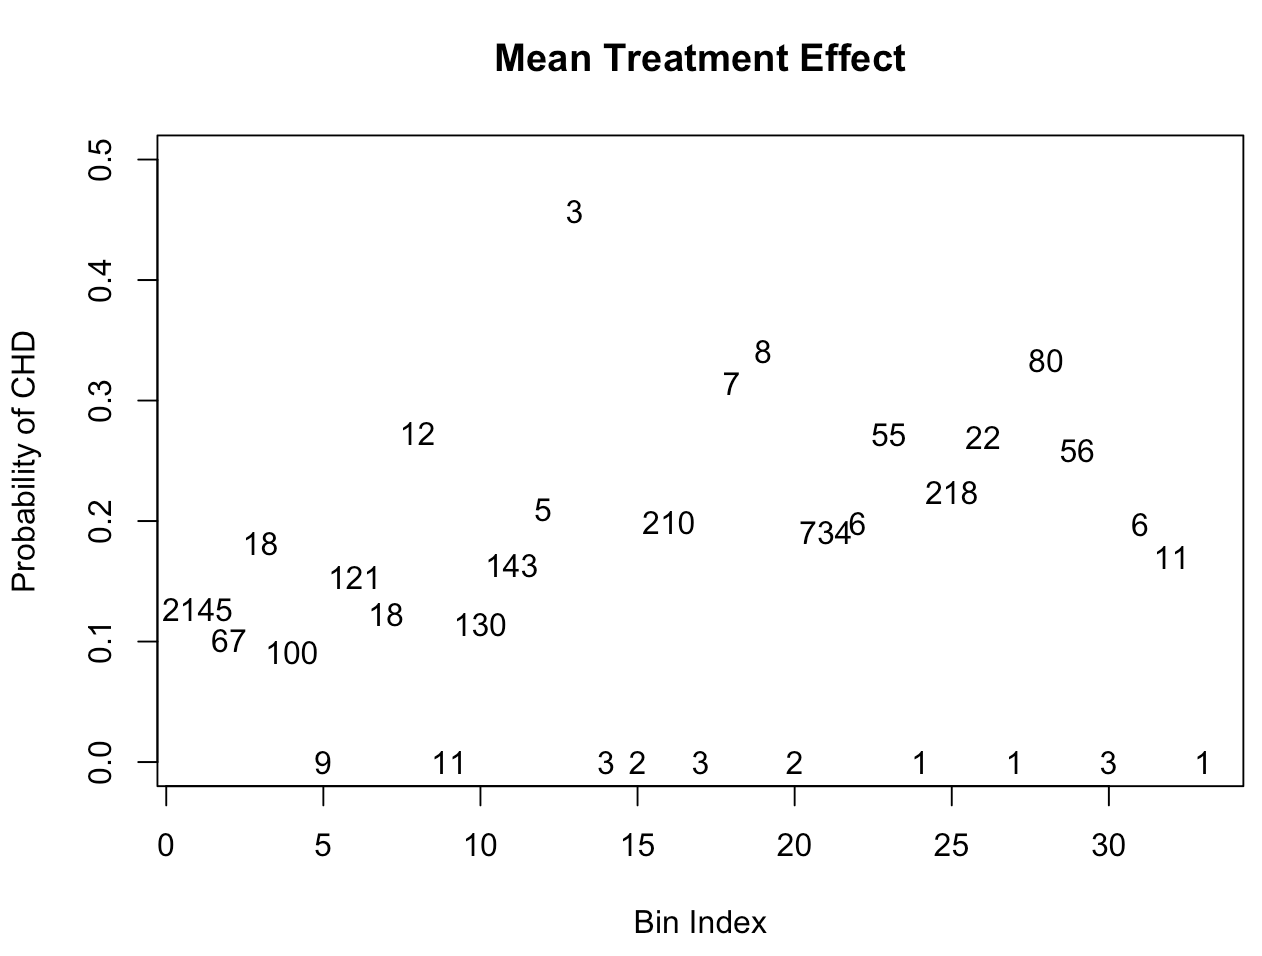
\includegraphics[width=0.5\linewidth]{./effect} 

}

\caption{Expected Outcome}\label{fig:fig2}
\end{figure}

\begin{figure}

{\centering 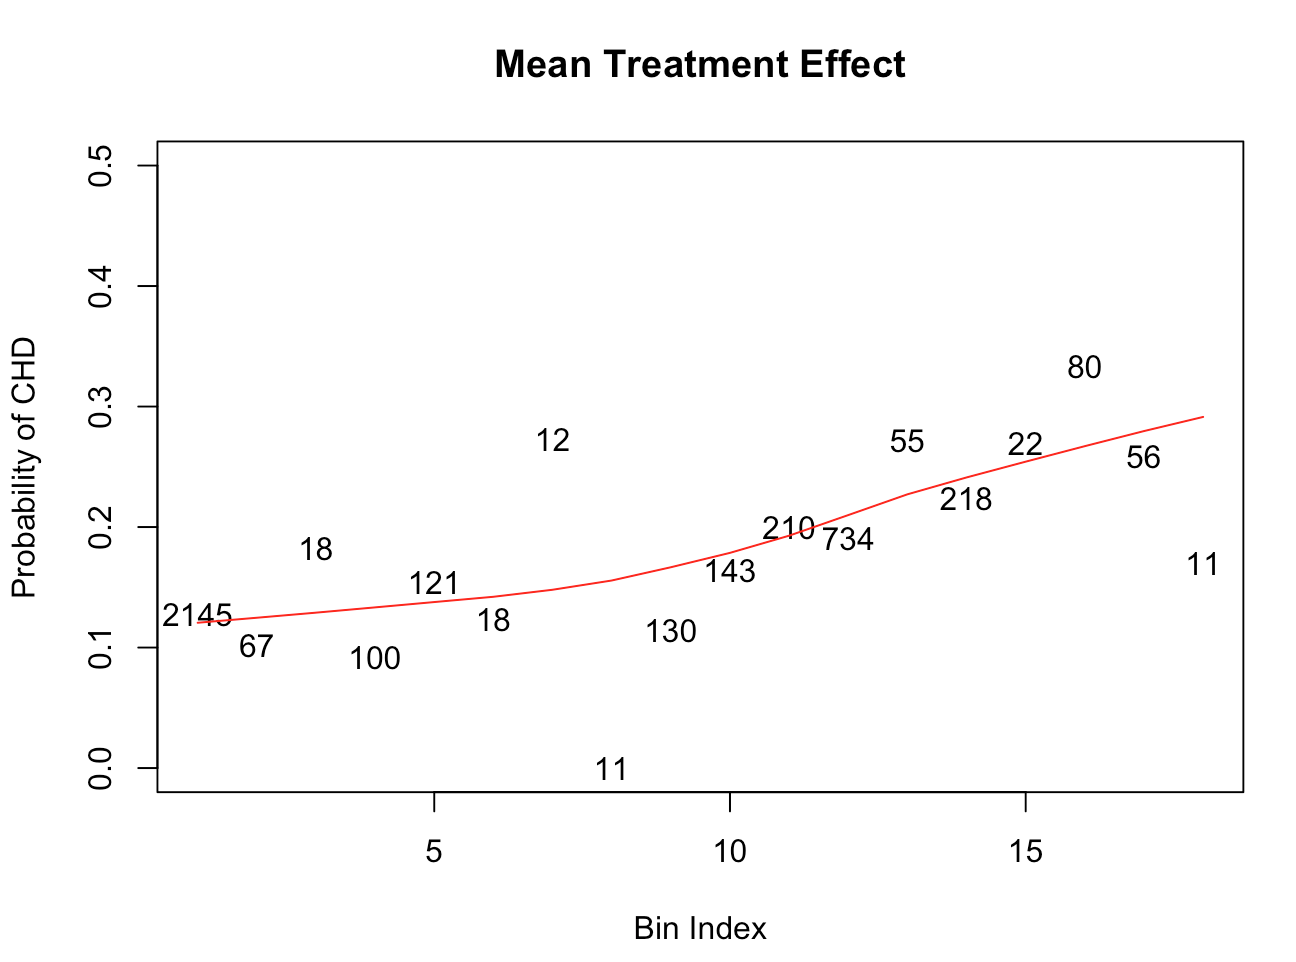
\includegraphics[width=0.5\linewidth]{./pos_violation2} 

}

\caption{Expected Outcome}\label{fig:fig3}
\end{figure}

\subsection{Statistical:}\label{statistical}

The probability of developing CHD in 10 years increases as theexposure
increases among subjects with similar baseline
covariatesForcigsPerDay∈{[}1,10), the exposure appears to have
a``protective effect''; this may be due to reporting bias /
practicalpositivity violationsFor more than 20 cigarettes, the exposure
effect starts to plateau,approaching a constant effect in risk of
CHDTMLE estimates more conservative than conditional mean \& IPTW

\subsection{Counterfactual:}\label{counterfactual}

The estimated effect of the exposure is the counterfactual probability
of CHD in 10 years under the exposure
category``cigsPerDay'',\(A_i \ i \in \{0,1,2,3\}\)), with the
assumptions thatW(age, sex, BMI, education, and diabetes) satisfy the
backdoorcriterion + positivity.Plausibility:As expected, we observed a
general increase in estimated risk ofCHD as the (binned) exposure
(cigsPerDay) is increased.Less plausible is the estimated reduction in
risk of CHD for \(cigsPerDay \in [0,10)\); this may be due to reporting
bias, or may infact be evidence for a ``protective effect'' of smoking
on risk of CHD.

\newpage

\subsection{Team Member Contribution}\label{team-member-contribution}

\subsubsection{Michael Attah}\label{michael-attah}

\begin{itemize}
\item Causal graph
\item Causal question
\item Estimation...
\item Interpretation?
\item etc
\end{itemize}

\subsubsection{Bianca Doone}\label{bianca-doone}

\begin{itemize}

\item Bootstrap confidence interval
\item Data Retrieval 
\item Causal graph
\item Causal question
\item Causal Parameter
\item Specify observed data and link to SCM
\item Descriptive table
\item Put together Table 1

\end{itemize}

\subsubsection{Casey Graham}\label{casey-graham}

\begin{itemize}
\item  Categorize covariates 
\item  Causal Parameter
\item  Conditional mean outcome
\item  IPTW
\item  Superlearner/TMLE
\item  Causal graph
\item  Causal question
\item  Statistical Estimand: G-comp
\item  etc

\end{itemize}

\subsubsection{Daniel Saunders}\label{daniel-saunders}

\begin{itemize}
\item  Data exploration
\item  Estimation...
\item  Interpretation?
\item  Causal graph
\item  Causal question
\item  etc

\end{itemize}

\subsubsection{Nutcha Wattanachit}\label{nutcha-wattanachit}

\begin{itemize}
\item  Background story 
\item  Descriptive table
\item  Causal graph
\item  Causal question
\item  Causal Parameter
\item  Specify observed data and link to SCM
\item  Identifiability: Randomization assumption
\item  Identifiability: Positivity assumption
\item  Statistical Estimand: G-comp

\end{itemize}

\subsection{References}\label{references}

Boston University \& the National Heart, Lung, \& Blood Institute,
Framingham Heart Study. 5 Dec. 2018:
\url{https://www.framinghamheartstudy.org}


\end{document}
